

An important property of dirac delta function that will be used at multiple ocassions in this solution is
\begin{align}
\displaystyle\int\limits_{-\infty}^{\infty} f(x)\delta(x-a)dx=f(a) \label{dec/2015/109/eq:dirac}
\end{align}
Given $X\sim N\brak{0,1}, Y\sim N(0,1)$
\begin{enumerate}
\item
\begin{align}
Cov(X,Y)=0\\
E\sbrak{XY}-E\sbrak{X}E\sbrak{Y}=0\\
E\sbrak{XY}=0\\
\displaystyle \int\limits_{-\infty}^{\infty} \int\limits_{-\infty}^{\infty}xyf_{XY}(x,y) dxdy=0
\end{align}
This doesn't imply independence. Counter example given below\\
Lets consider a case where $X$ and $Y$ are dependent based on the following relation, $Y$ being independent of $K$
\begin{align}
X=KY \label{dec/2015/109/eq:case}
\end{align}
PMF for $K$ is given as
\begin{align}
p_K(k)=
\begin{cases}
\frac{1}{2} &k=1\\
\frac{1}{2} & k=-1\\
0 & \text{otherwise}
\end{cases}
\end{align}
A simulation is given below, Y is gaussian, then X also follows gaussian
\begin{figure}[!ht]
\centering
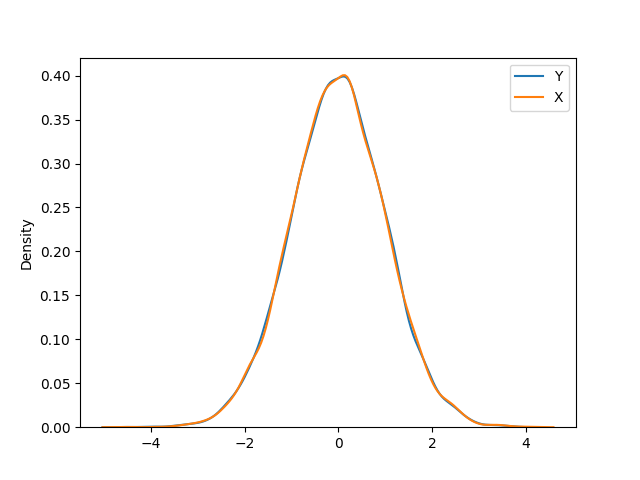
\includegraphics[width=\columnwidth]{solutions/2015/dec/109/figure/fig.png}
\caption{X and Y, if Y is normal}
\label{fig:dec/2015/109/plot}
\end{figure}
Theoretically it can be proved in the following manner,
Since $K$ and $Y$ are independent
\begin{align}
f_X(x)&=\pr{K=1}f_Y(x)+\pr{K=-1}f_Y(-x)\\
&=\frac{1}{2}\brak{f_Y(x)+f_Y(-x)}\\
&=f_Y(x)
\end{align}
Therefore, $X$ follows identical but not independent distribution as $Y$, An alternative proof is given below as a proof for marginal probability\\
Now consider that $X$ is normally distributed, we will establish $Y$ is also normally distributed.
The joint probability distribution is therefore
\begin{align}
f_{XY}(x,y)&=f_{X|Y}(x|y)f_X(x)\nonumber \\
&=f_X(x)\frac{1}{2}(\delta(x+y)+\delta(x-y))\label{dec/2015/109/eq:counter}
\end{align}
The marginal probability distribution function for $X$ is given as
\begin{align}
\int\limits_{-\infty}^{\infty}f_X(x)\frac{1}{2}(\delta(x+y)+\delta(x-y)) dy
\end{align}
Using \eqref{dec/2015/109/eq:dirac}, we get
\begin{align}
\int\limits_{-\infty}^{\infty}f_X(x)\frac{1}{2}(\delta(x+y)+\delta(x-y))dy=f_X(x)
\end{align}
We know that $X\sim N(0,1)$, $f_X(x)$ represents gaussian probability distribution function.\\
Futher, using symmetry of \eqref{dec/2015/109/eq:case}, we can establish that marginal distribution of $Y$ is gaussian. Here is a proof anyways
\begin{align}
f_Y(y)=\int\limits_{-\infty}^{\infty}f_X(x)\frac{1}{2}(\delta(x+y)+\delta(x-y)) dx
\end{align}
Using \eqref{dec/2015/109/eq:dirac}, we get
\begin{align}
f_Y(y)=\frac{1}{2}\brak{f_X(y)+f_X(-y)}=f_X(y)
\end{align}
Since $Y$ has identical probability distribution function, $Y\sim N(0,1)$\\
The covariance is given as
\begin{align}
&Cov(X,Y)=E[XY]-E[X]E[Y]=E[XY]\\
&E[XY]=\int\limits_{-\infty}^{\infty}\int\limits_{-\infty}^{\infty}xyf_{XY}(x,y) dy dx
\end{align}
\begin{align}
=\int\limits_{-\infty}^{\infty}\int\limits_{-\infty}^{\infty}xyf_X(x)\frac{1}{2}(\delta(x+y)+\delta(x-y)) dy dx\\
=\int\limits_{-\infty}^{\infty} xf_X(x)\int\limits_{-\infty}^{\infty}y\frac{1}{2}(\delta(x+y)+\delta(x-y)) dy dx
\end{align}
Using \eqref{dec/2015/109/eq:dirac}
\begin{align}
E[XY]=\int\limits_{-\infty}^{\infty}xf_X(x)\frac{1}{2}(x-x)dx=0
\end{align}
\item
Defining the following matrices/vectors
\begin{table}[h!]
\centering
\begin{tabular}{ |c|c|} 
\hline
\textbf{vector/matrix} & \textbf{expression} \\
\hline&\\[-1em]
$\boldsymbol{Z}$& $\begin{pmatrix} X &Y\end{pmatrix}^\top$\\[2pt]
\hline&\\[-1em]
$\boldsymbol{C}$&$\begin{pmatrix} a &b\end{pmatrix}^\top$  \\[2pt]
\hline&\\[-1em]
$\boldsymbol{\mu}$&$\begin{pmatrix} 0 &0\end{pmatrix}^\top$  \\[2pt]
\hline&\\[-1em]
$\boldsymbol{\Sigma}$&$\begin{pmatrix}1&\rho\\\rho&1\end{pmatrix}$ \\
\hline
\end{tabular}
\caption{vectors/matrices and their expressions}
\label{dec/2015/109/table1}
\end{table}
Given
\begin{align}
\boldsymbol{C^\top Z}\sim N\brak{0,a^2+b^2}
\end{align}
Since this is true for all $a$ and $b$, it is equivalent to $X$ and $Y$ being jointly gaussian
\begin{align}
\boldsymbol{Z}\sim N(\boldsymbol{\mu},\boldsymbol{\Sigma})
\end{align}
For correlated random variables $X$ and $Y$ in bivariate normal distribution, we have
\begin{align}
\sigma_{Z}^2=\displaystyle\sum_{i,j}\Sigma_{ij}\\
a^2+b^2=a^2+b^2+2\rho ab\\
\therefore \rho=0\label{dec/2015/109/eq:rho}
\end{align}
The joint distribution is given as
\begin{align}
f_{\boldsymbol{Z}}(x,y)=\frac{\text{exp}\brak{-\frac{1}{2}\brak{\boldsymbol{z-\mu}}^\top\boldsymbol{\Sigma}^{-1}\brak{\boldsymbol{z-\mu}}}}{\sqrt{(2\pi)^2\abs{\boldsymbol{\Sigma}}}}\\
f_{\boldsymbol{Z}}(x,y)=\frac{\text{exp}\brak{-\frac{1}{2}{\begin{pmatrix} x &y\end{pmatrix}} I_2{\begin{pmatrix} x &y\end{pmatrix}}^\top}}{\sqrt{(2\pi)^2}}
\end{align}
Where $I_2$ is the identity matrix of order 2
\begin{align}
f_{\boldsymbol{Z}}(x,y)=\frac{\text{exp}\brak{-\frac{1}{2}{\begin{pmatrix} x &y\end{pmatrix}} {\begin{pmatrix} x &y\end{pmatrix}}^\top}}{\sqrt{(2\pi)^2}}\\
f_{\boldsymbol{Z}}(x,y)=\frac{\text{exp}\brak{-\frac{1}{2}\brak{x^2+y^2}}}{\sqrt{(2\pi)^2}}=f_X(x)f_Y(y)
\end{align}
$\therefore$ \textbf{Option(2) is correct}, A simulation for bivariate gaussian is given below
\begin{figure}[!ht]
\centering
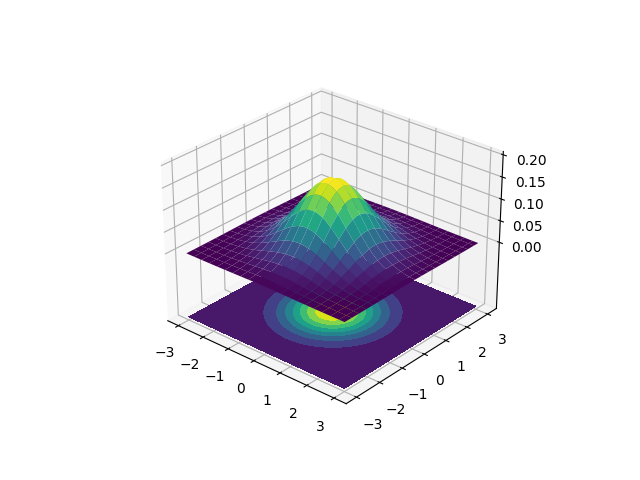
\includegraphics[width=\columnwidth]{solutions/2015/dec/109/figure/plot.png}
\caption{bivariate gaussian while 0 mean vector and identity covariance matrix}
\label{dec/2015/109/plot}
\end{figure}
\item
\begin{align}
\pr{X\le 0, Y\le0}=\frac{1}{4}
\end{align}
This doesn't imply independence, it can be true even for dependent $X$ and $Y$, the counter example is \eqref{dec/2015/109/eq:counter}, the joint probability function is symmetric across all 4 quadrants
\begin{align}
\therefore \pr{X\le 0, Y\le0}=\frac{1}{4}
\end{align}
Alternatively, here is proof 
\begin{align}
\pr{X\le 0}=F_X(0)=\frac{1}{2} \label{dec/2015/109/eq:pr1}
\end{align}
Using \eqref{dec/2015/109/eq:case}
\begin{align}
\pr{Y\le 0|X\le 0}=\frac{1}{2} \label{dec/2015/109/eq:pr2}
\end{align}
Using \eqref{dec/2015/109/eq:pr1} and \eqref{dec/2015/109/eq:pr2}
\begin{align}
\pr{X\le 0, Y\le0}=\frac{1}{4}
\end{align}
\item
\begin{align}
E\sbrak{e^{itX+isY}}=E\sbrak{e^{itX}}E\sbrak{e^{isY}}\\
E\sbrak{e^{itX+isY}}=\varphi_X(t)\varphi_Y(s) \label{dec/2015/109/eq:inde}
\end{align}
The inverse is given as
\begin{align}
f_{XY}(x,y)=\frac{1}{4\pi^2}\displaystyle \int\limits_{-\infty}^{\infty} \int\limits_{-\infty}^{\infty} e^{-itX-isY}E\sbrak{e^{itX+isY}}ds dt
\end{align}
Using \eqref{dec/2015/109/eq:inde}
\begin{align}
f_{XY}(x,y)&=\frac{1}{4\pi^2}\displaystyle \int\limits_{-\infty}^{\infty} \int\limits_{-\infty}^{\infty} e^{-itX-isY}\varphi_X(t)\varphi_Y(s) ds dt\\
&f_{XY}(x,y)=f_X(x)f_Y(y)
\end{align}
$\therefore$ \textbf{Option(4) is correct}
\end{enumerate}


